\chapter{Model Training and Optimization}
\label{ch:chapter06}
 
%
% Section: 6 - Intro
%

To automatically classify software usage purposes, \ac{Sci-BERT} multi-class model has been trained and tested using \ac{SoMeSci} data set. The model has been trained in various training scenarios to determine conditions that leads to improved performance. The training scenarios considered the effect of context information  and the impact of including or excluding parts of \ac{SoMeSci} data set on the classifier’s performance.\\
 
In addition, \emph{software-purpose} classification performance has also been investigated by removing \emph{mention-type} and \emph{software-type} classifiers from cascades of classifier modules shown on the figure 5.6.  Further more, the impact of using another variant of BERT model, \ac{Bio-BERT}, on classifier’s performance  has also been investigated. \\

Finally, results from all training scenarios have been discussed and best performing model has been selected based on the results of investigation.

\section{The impact of labeled data}
\label{sec:chapter06:exclusion}

As described in the table 4.1 before, the \ac{SoMeSci} dataset is composed of 4 different sets of articles: \emph{PLoS-methods, PubMed-full text,  PLoS-sentences} and \emph{creation-sentences}. Since only articles in the  \emph{PLoS-methods} and \emph{PubMed-full text} are annotated with software usage purpose labels, it was desired to evaluate weather including \emph{PLoS/Creation} sentences, would result in improved performance of \emph{software-purpose} classification.  \\

The results of evaluation indicates that including \emph{ PLoS-sentences} and \emph{creation-sentences} in the training dataset, definitely improved the overall performance for classification of software, but not for software usage purpose. Figure 6.1 below shows total F-score for \emph{software classification} over test and development sets is improved with the addition of \emph{PLoS/Creation} sentences in the training dataset. \\

\begin{figure}[htbp]
	\centering
	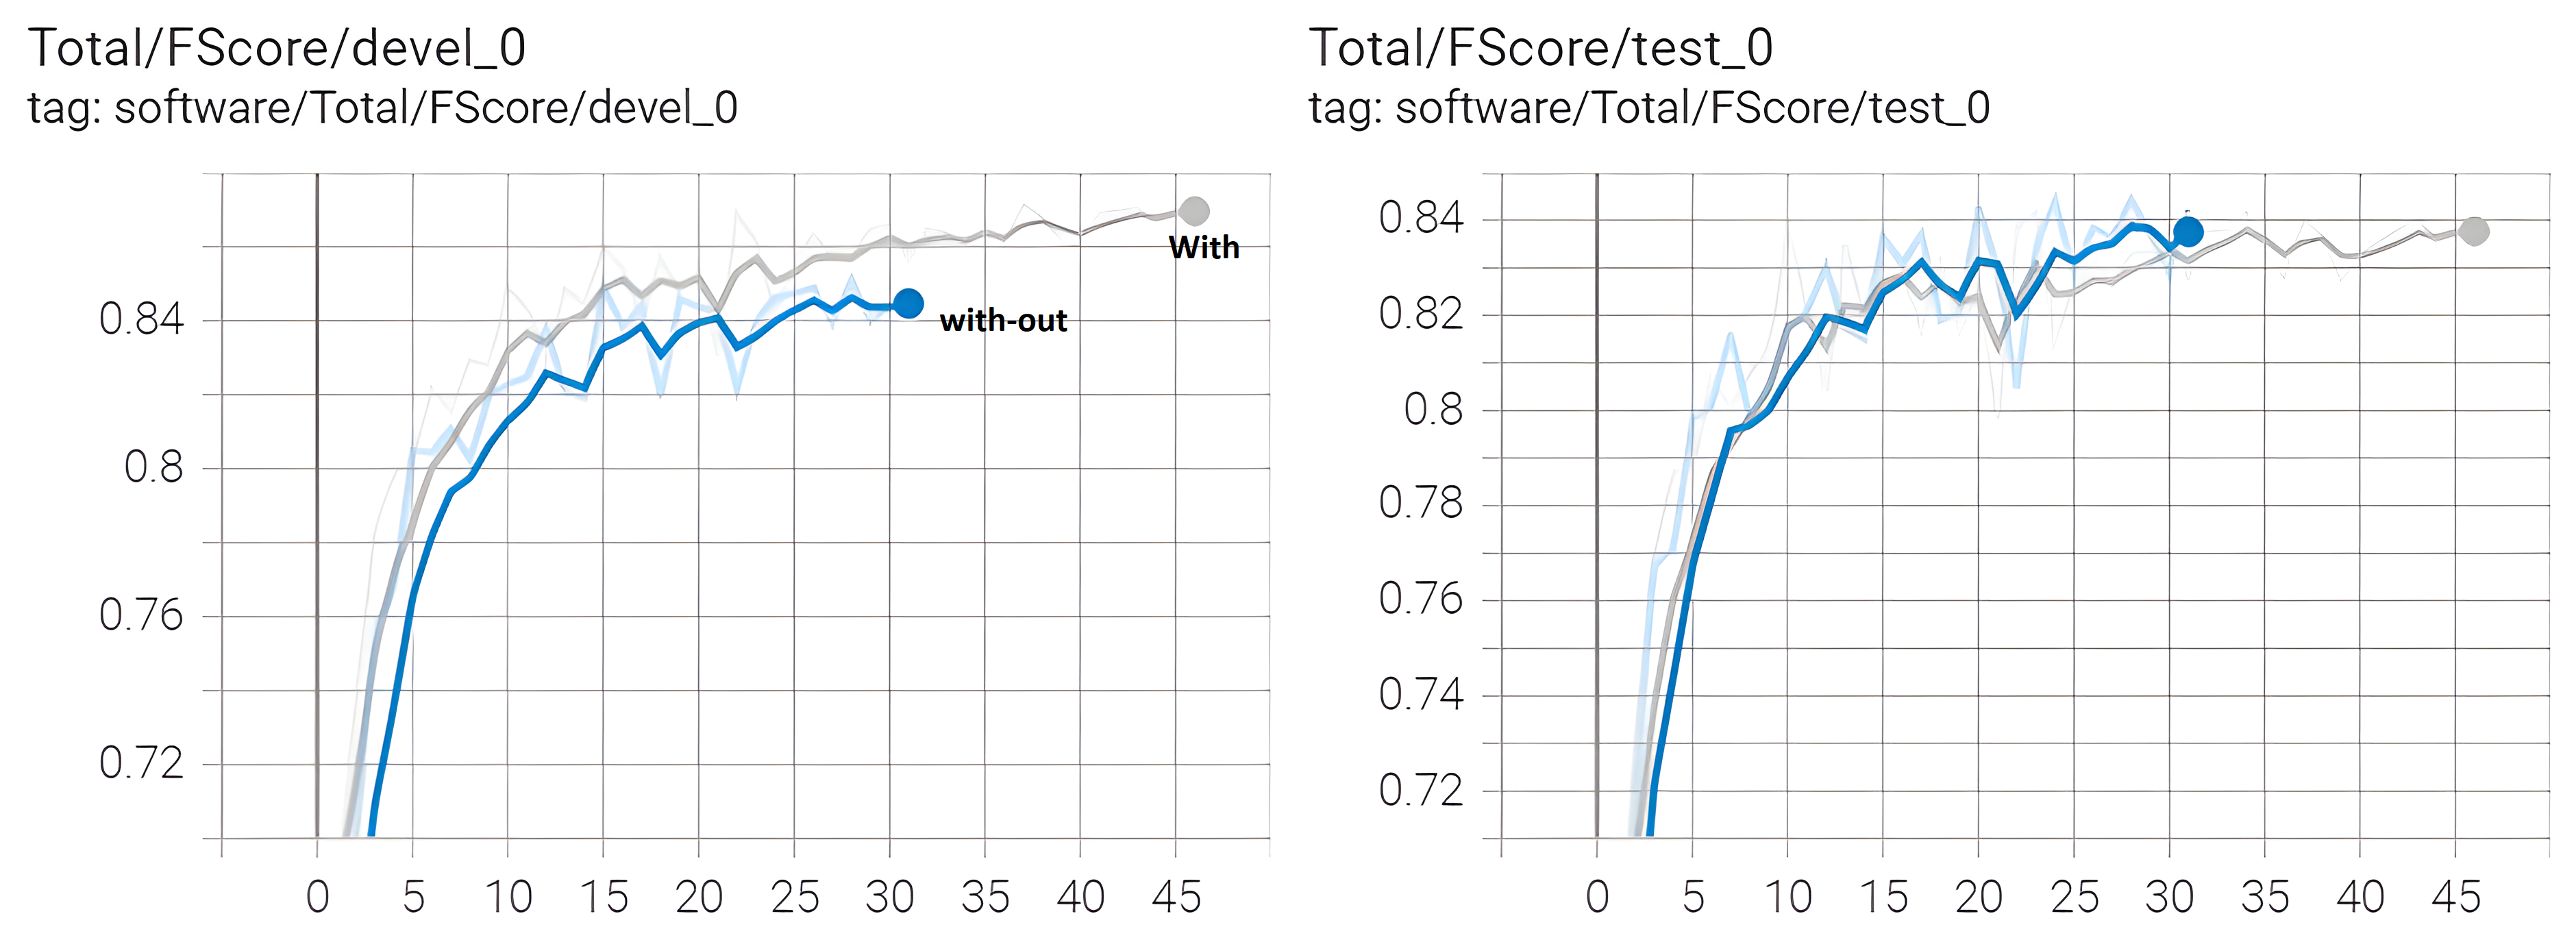
\includegraphics[width=.86\textwidth]{4.graphics/figures/ch_6/1.with_sent_vs_without/HD/TotalFscoresoftware}
	\caption{Software classification (Total) F1-score over devl.(left) and test(right) sets shows improvement when \emph{Creation/PLoS} sentences are included in the training dataset.}
	\label{fig:chapter06:with}
\end{figure}


In contrast, the total F-score performance for \emph{software-purpose} classification is diminished when trained with \emph{PLoS} and \emph{Creation} sentences as shown on the Figure 6.2. \\

\begin{figure}[htbp]
	\centering
	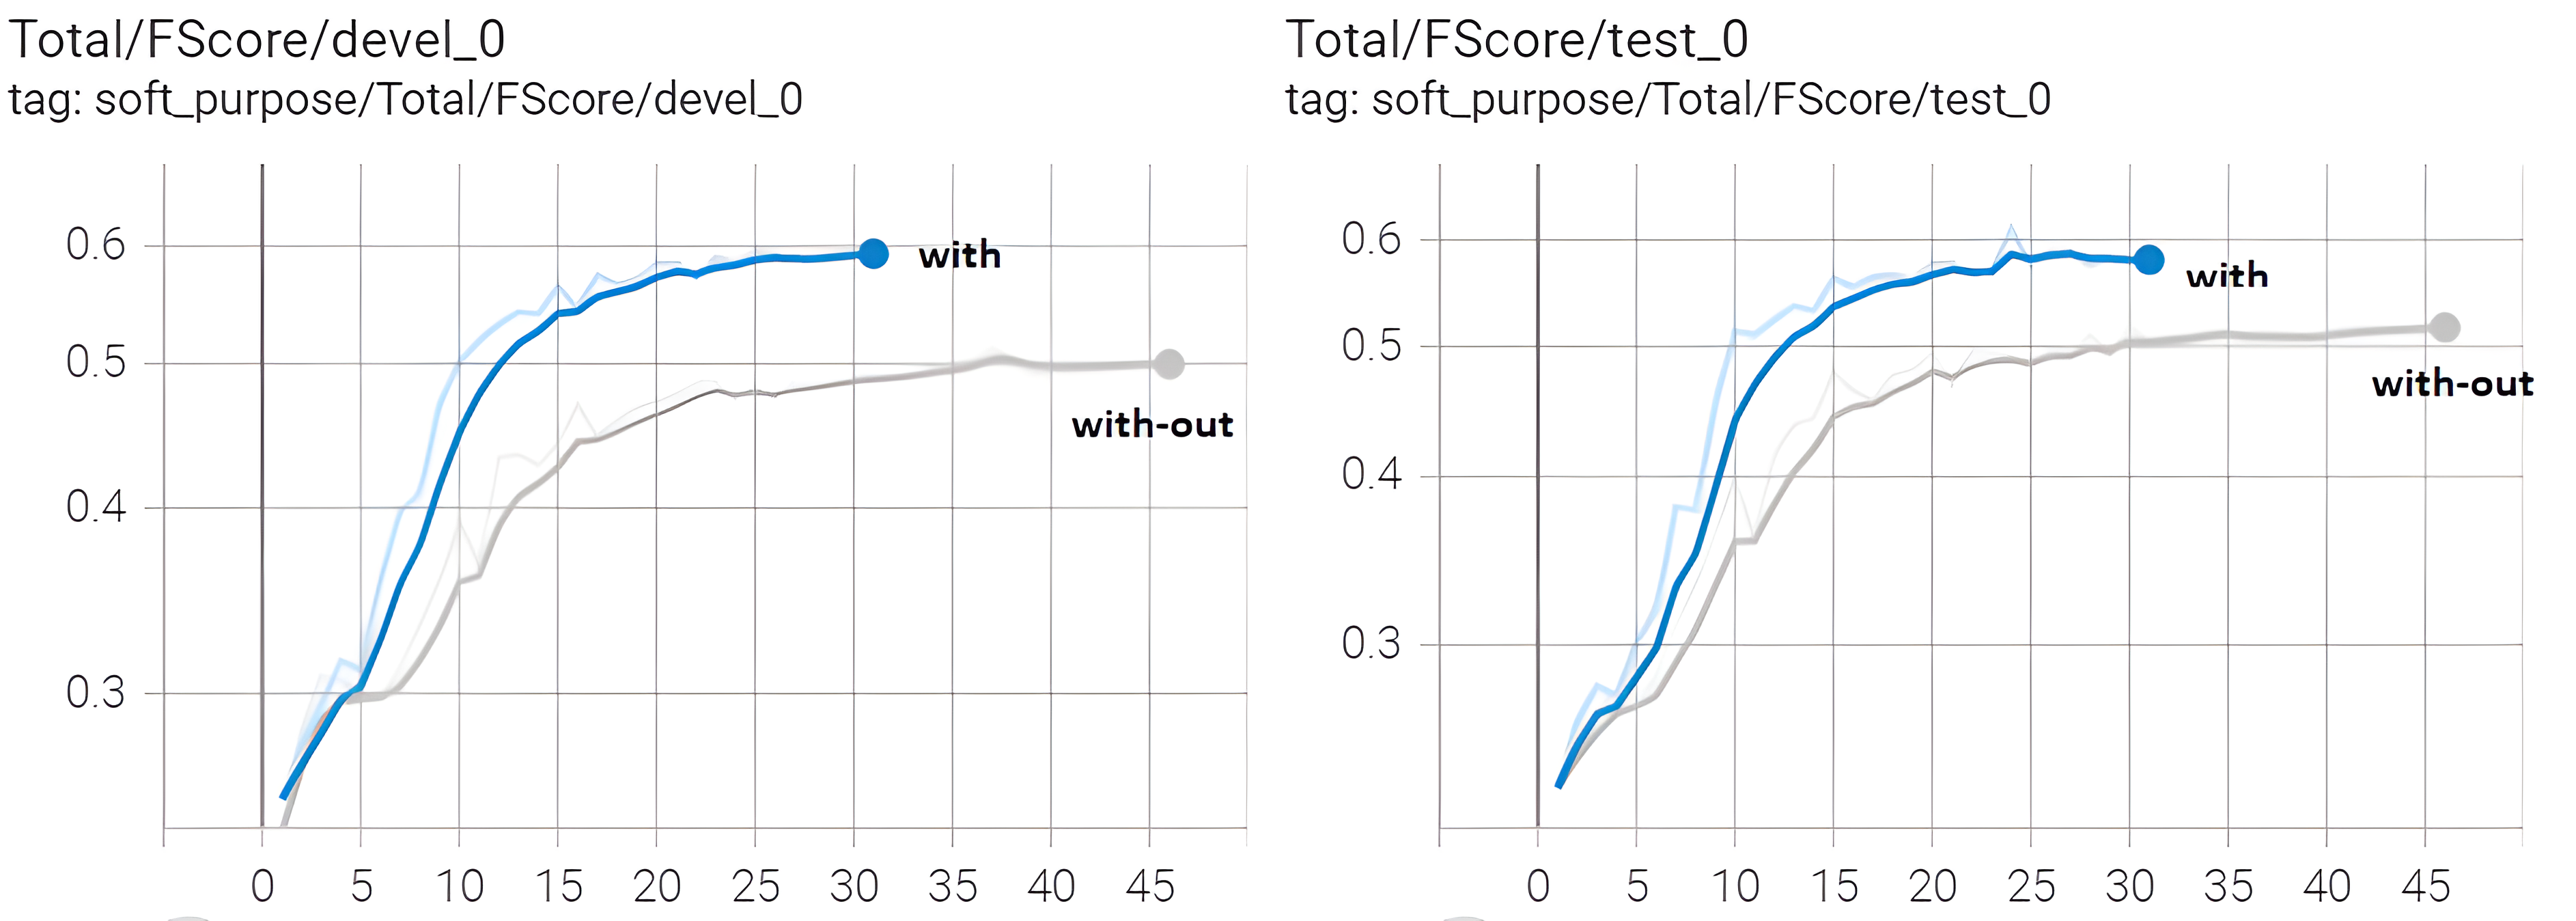
\includegraphics[width=1\textwidth]{4.graphics/figures/ch_6/1.with_sent_vs_without/HD/Total_Fscore_software_purpose}
	\caption{Software purpose classification (Total) F1-score degrades for devl. set (left) and test set (right) when \emph{Creation/PLoS} sentences are included in the training dataset.}
	\label{fig:chapter06:withvswitout}
\end{figure}


\begin{table}[ht]
	\centering
	\caption{Evaluation of software purpose classifier's performance with(+) and without(-) \emph{Creation/PLoS}sentences in the training data set.}
	\begin{tabular*}{0.75\textwidth}{@{\extracolsep{\fill}}  l  l l  l l l } %l left align , c- center
		\hline
		Software Purpose & Metric & Dev+        & Dev-     & Test+  &Test- \\
		\hline 
		Analysis         & F     & 0.64        & 0.71     &0.65     &0.69   \\
		                 & P     & 0.61        & 0.71     &0.60     &0.66   \\
		                 & R     & 0.68        & 0.71     &0.72     &0.73   \\
		\hline
		Data-Collection  & F     & 0.26        &  0.32    & 0.26    & 0.34  \\
					     & P     & 0.25        &  0.33    & 0.22    & 0.30  \\
						 & R     & 0.28        &  0.31    & 0.30    & 0.31  \\		
		
		\hline
		Pre-Processing   & F     & 0.41        &  0.45    & 0.49    & 0.57  \\
						 & P     & 0.36        &  0.37    & 0.45    & 0.49  \\
						 & R     & 0.48        &  0.56    & 0.58    & 0.67  \\
		\hline
		Modeling         & F     & 0.25        &  0.54    & 0.30    & 0.44  \\
					     & P     & 0.27        &  0.54    & 0.28    & 0.42  \\
						 & R     & 0.24        &  0.55    & 0.30    & 0.46  \\
	
		\hline
		Programming      & F     & 0.27        &  0.42    & 0.23    & 0.42  \\
						 & P     & 0.28        &  0.34    & 0.24    & 0.36  \\
						 & R     & 0.27        &  0.55    & 0.23    & 0.51  \\
		
		\hline
		Simulation      & F     & 0.00        &  0.38    & 0.00    & 0.00 \\
						& P     & 0.00        &  0.88    & 0.00    & 0.00  \\
						& R     & 0.00        &  0.25    & 0.00    & 0.00  \\
		
		\hline
		Stimulation     & F     & 0.46        &  0.59    & 0.24    & 0.26 \\
						& P     & 0.40        &  0.76    & 0.21    & 0.24  \\
						& R     & 0.48        &  0.45    & 0.28    & 0.22  \\
		
		\hline
		Visualization   & F     & 0.48        &  0.59    & 0.52    & 0.58  \\
						& P     & 0.46        &  0.59    & 0.46    & 0.54  \\
						& R     & 0.51        &  0.61    & 0.56    & 0.62  \\
		\hline
		Total (software Purpose)	& F     & 0.27        &  0.58*    & 0.30    & 0.54*  \\
								& P     & 0.26        &  0.62*    & 0.26    & 0.56*  \\
								& R     & 0.31        &  0.55*    & 0.32    & 0.65*  \\
		\hline
		Total (software) 	& F     &  0.86*       & 0.84     & 0.83    & 0.83  \\
						    & P     &  0.83*       & 0.82     & 0.77    & 0.79*  \\
						    & R     &  0.90*       & 0.86     & 0.90*    & 0.87  \\
		\hline
	\end{tabular*}
\end{table}%

Software purpose classifier's performance when trained with \emph{Creation/PLoS} sentences versus  without is summarized on the table 6.1. Overall, as shown in table 6.1, it is observed that including a dataset that lacks software purpose annotation harms \emph{software-purpose} classifier’s performance. Since the main objective of this thesis is software purpose classification, for subsequent steps of analysis the Sci-BERT model has been trained only with datasets of \emph{PLoS-methods} and \emph{PubMed-full text} by excluding \emph{Creation/PLoS} sentences. \\


\section{The impact of larger context}
\label{sec:chapter06:largercontext}

Scientific papers like any other well written documents, have a sequential structure that form abstraction at various levels such as sentence, paragraphs, sections, chapters, etc. These levels of abstractions often determine the meaning of words because each level of abstraction or context conveys a valuable information \citep{ghosh2016contextual}. \\

Likewise, contextual information helps to determine the correct purpose of use of a software. Therefore for each sentence in a text of scientific articles of training data set, various range of neighboring sentences have been incorporated to provide a contextual information. Typically 2 adjacent sentences before a sentence, after a sentence, and before \& after a sentence have been considered. Further more, a context as broad as the whole paragraph has also been considered. \\

Excerpt of the python code for reading neighboring sentences for context is listed on the \emph{appendix-E} and the complete source code can be found on the git-hub.\footnote{\url{https://github.com/BeTKH/SoMeNLP/blob/contxt2Sentcs_wo/somenlp/NER/data_handler.py}}\\

Evaluation of a Sci-BERT model with a broader context of two adjacent sentences, from left and right, improved software purpose classification F-score as shown on the figure 6.3 below. 

\begin{figure}[htbp]
	\centering
	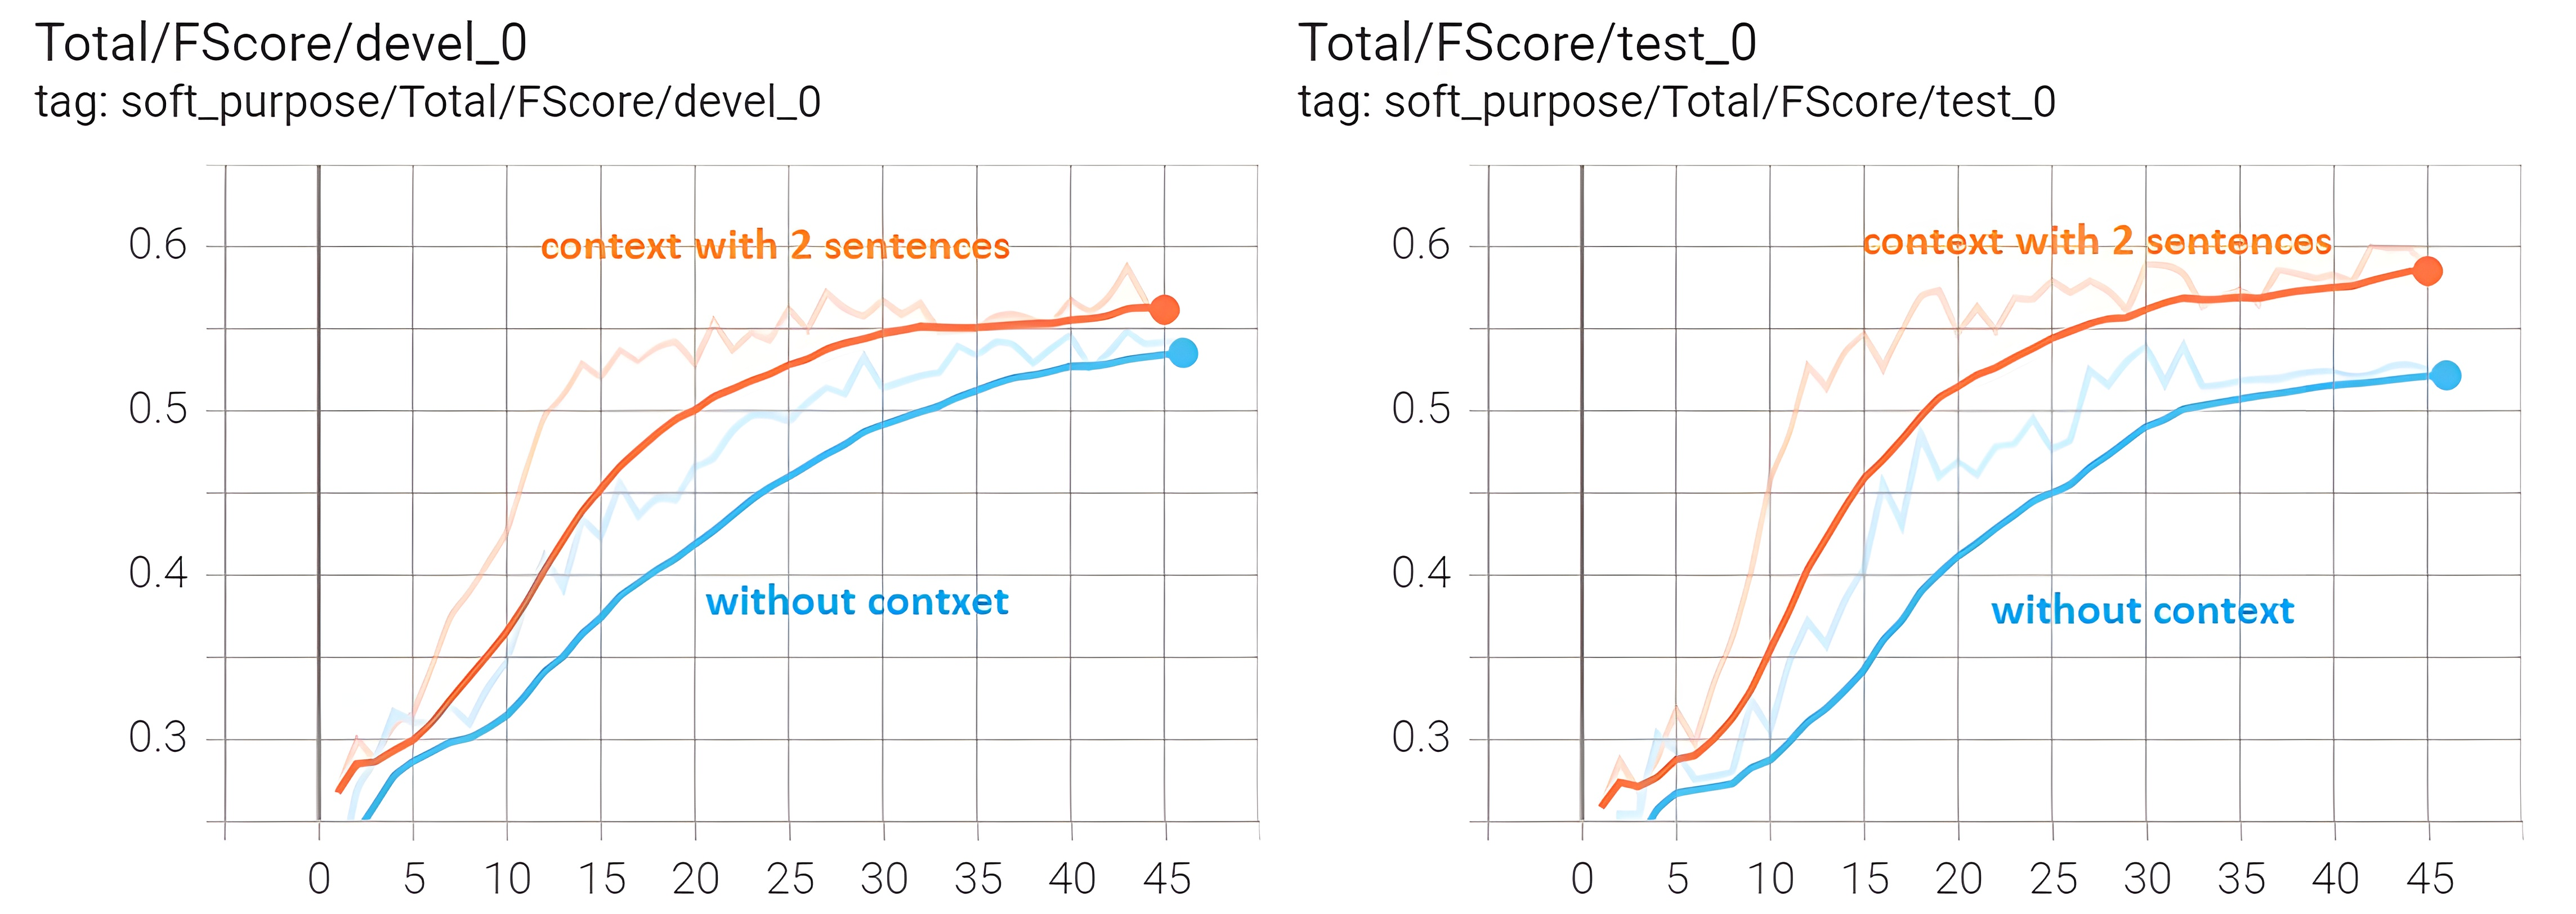
\includegraphics[width=.86\textwidth]{4.graphics/figures/ch_6/2.left_context_vs_right/HD/braoderContextFscore}
	\caption{Software purpose classification (Total) F1-score improves for devl. set (left) and test set (right) when trained with a broader context of two adjacent sentences compared to without context (blue).}
	\label{fig:chapter06:withvswithout}
\end{figure}

\subsection{Left vs Right Context within a paragraph}
\label{sec:chapter06:leftvsright}

In addition to a broader context, it was also desired to determine which part of context, left versus right, is more important for the software purpose classification. Left context refers to sentences prior to a given sentence with in  a paragraph and right context refers to sentences that lie right after a given sentence. To determine the impact of neighboring context on the software-purpose classification performance, two adjacent sentences from the left and right has been used to train the Sci-BERT model.  \\

According to the classification's F1-Score, sentences from the left are more important than the sentences on the right side. In addition, the 2-sentences from the left (2,0) has more significance over 2-sentences from left-and-right (2,2) as shown on the table 6.2. This indicates that the Sci-BERT classifier is not benefited any more by including the right context(0,2) or both contexts(2,2) as portrayed on the figure 6.4. below. 

\begin{figure}[htbp]
	\centering
	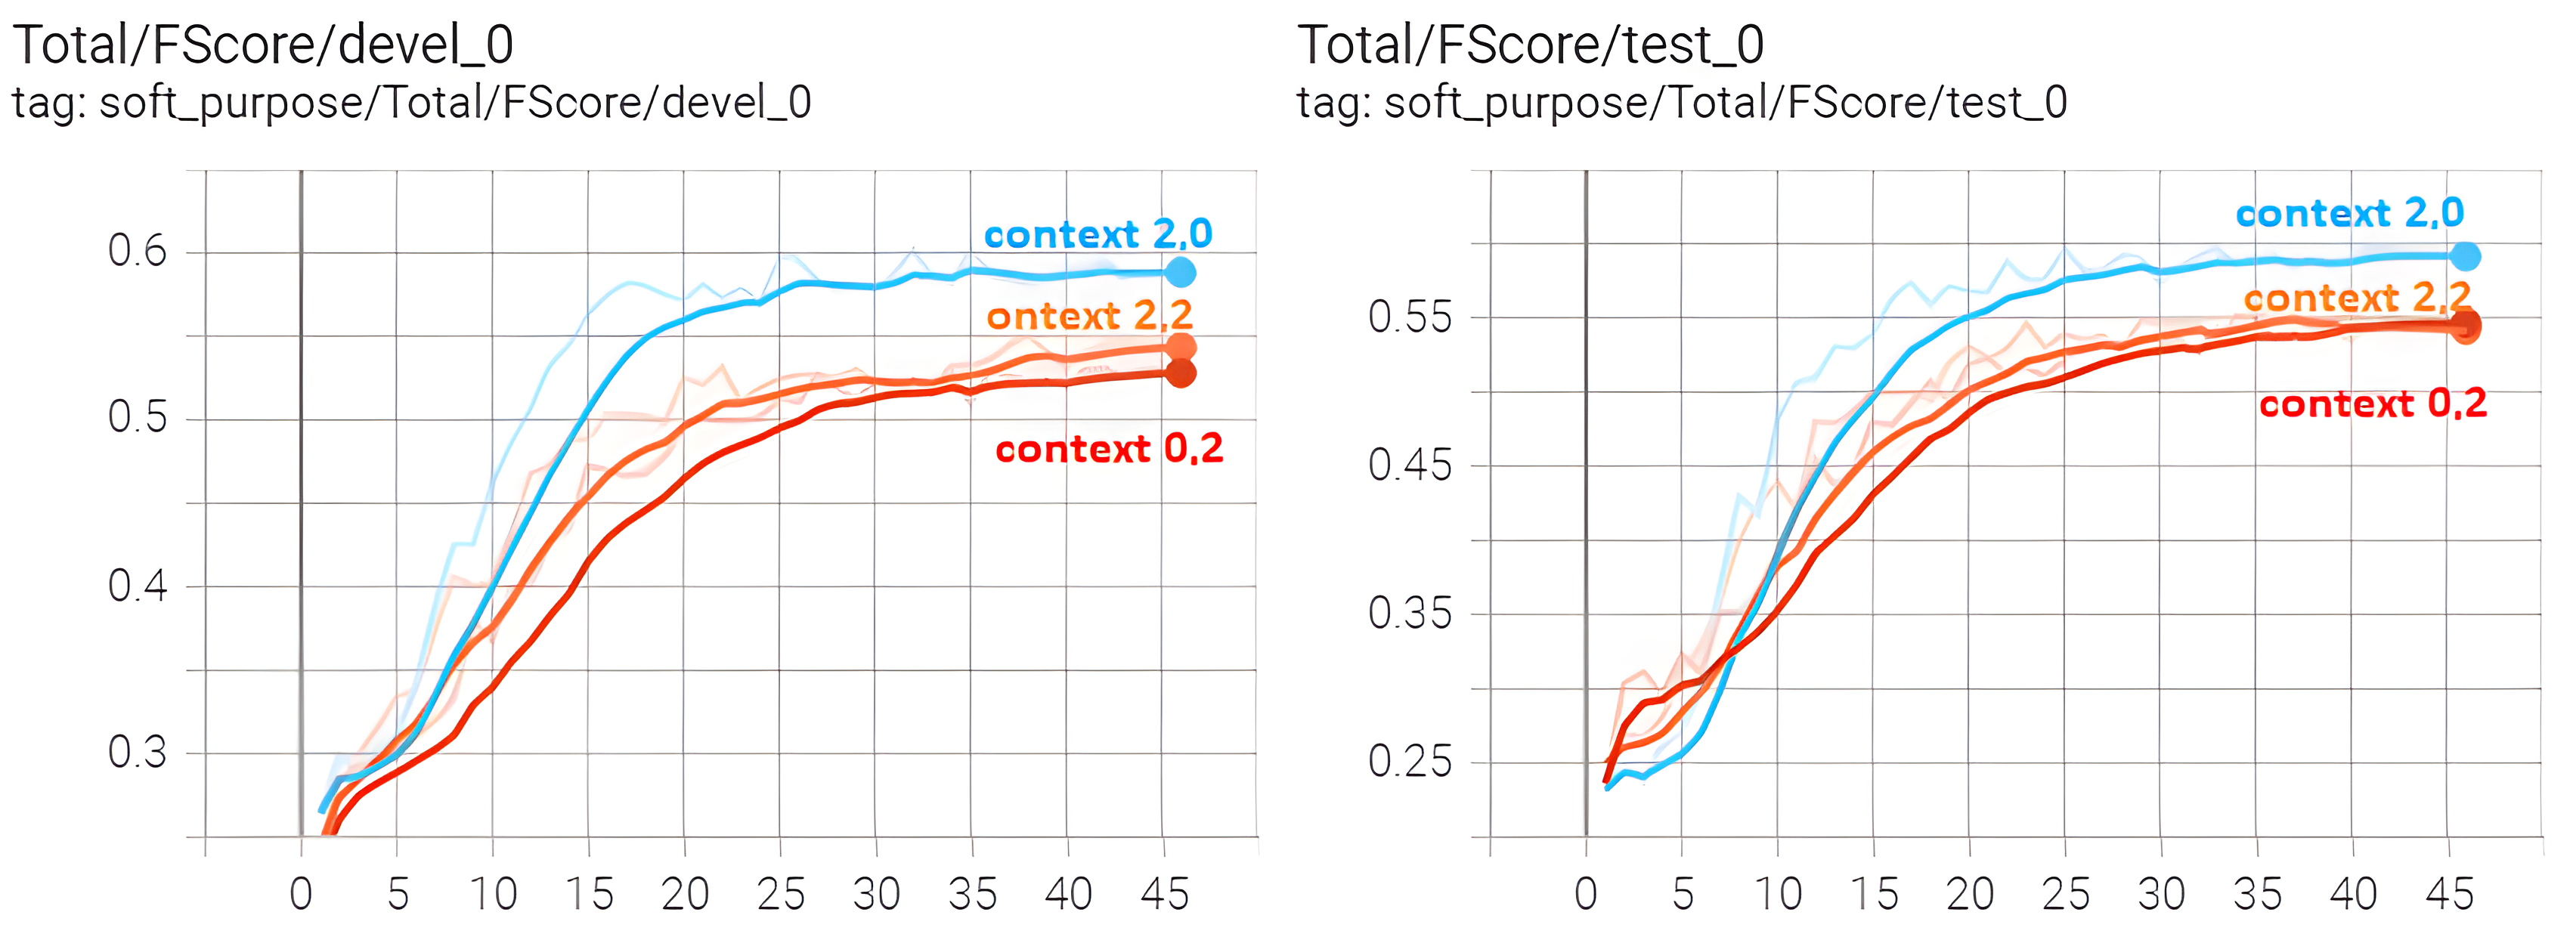
\includegraphics[width=.86\textwidth]{4.graphics/figures/ch_6/2.left_context_vs_right/HD/left_both_right_hd}
	\caption{Software purpose classification (Total) F1-score performance for devl. set (left) and test set (right) when trained with left-context (2,0) has superior performance over right-context (0,2) as well as combined left-and-right-context (2,2).}
	\label{fig:chapter06:l-r-softwarepurpose}
\end{figure}

\begin{table}[ht]
	\centering
	\caption{Comparison of 4-cascade multi-class Sci-BERT software purpose classifier's F-score, Precision and Recall performance for various levels of context information.}
	\begin{tabular*}{1\textwidth}{@{\extracolsep{\fill}}  l  l l  l l r r r } %l left align , c- center
		\hline
		Software Purpose & Metric & Dv.(2,0)        & Dv.(0,2)     & Dv.(2,2)  &Tst(2,0) & Tst(0,2) & Tst(2,2) \\
		\hline 
		Analysis & F     & 0.72        & 0.66     &0.69     &0.70    &0.68     &0.69 \\
				 & P     & 0.72        & 0.64     &0.68     &0.65    &0.63     &0.64\\
		         & R     & 0.73        & 0.68     &0.71     &0.76    &0.74     &0.74\\
		\hline
		Data-Collection  & F     & 0.29        &  0.31    & 0.25    & 0.38   &0.20     &0.31\\
		                 & P     & 0.29        &  0.29    & 0.24    & 0.38   &0.22     &0.32\\
		                 & R     & 0.29        &  0.32    & 0.25    & 0.39   &0.20     &0.29\\		
		
		\hline
		Pre-Processing   & F     & 0.45        &  0.45    & 0.41    & 0.58   &0.58     &0.52\\
						 & P     & 0.36        &  0.36    & 0.37    & 0.49   &0.48     &0.44\\
						 & R     & 0.59        &  0.59    & 0.52    & 0.73   &0.73     &0.64\\
		\hline
		Modeling         & F     & 0.50        &  0.50    & 0.38    & 0.42   &0.42     &0.31\\
						 & P     & 0.42        &  0.42    & 0.41    & 0.37   &0.37     &0.30\\
						 & R     & 0.62        &  0.62    & 0.35    & 0.48   &0.48     &0.31\\
		
		\hline
		Programming      & F     & 0.42        &  0.41    & 0.44    & 0.41   &0.33     &0.42\\
						 & P     & 0.32        &  0.32    & 0.34    & 0.36   &0.28     &0.37\\
						 & R     & 0.61        &  0.57    & 0.64    & 0.48   &0.42     &0.51\\
		
		\hline
		Simulation      & F     & 0.24        &  0.00    & 0.25    & 0.00   &0.00     &0.00\\
						& P     & 0.33        &  0.00    & 0.39    & 0.00   &0.00     &0.00\\
						& R     & 0.19        &  0.00    & 0.20    & 0.00   &0.00     &0.00\\
		
		\hline
		Stimulation     & F     & 0.47        &  0.34    & 0.39    & 0.34   &0.41     &0.24\\
						& P     & 0.56        &  0.42    & 0.51    & 0.26   &0.37     &0.20\\
						& R     & 0.41        &  0.32    & 0.31    & 0.50   &0.47     &0.32\\
		
		\hline
		Visualization   & F     & 0.58        &  0.36    & 0.54    & 0.60   &0.40     &0.50\\
						& P     & 0.60        &  0.35    & 0.54    & 0.57   &0.41     &0.46\\
						& R     & 0.56        &  0.38    & 0.53    & 0.64   &0.41     &0.54\\
		\hline
		Total	        & F     & 0.58        &  0.53    & 0.55    & 0.59   &0.54     &0.55\\
						& P     & 0.57        &  0.51    & 0.54    & 0.54   &0.51     &0.51\\
						& R     & 0.62        &  0.55    & 0.57    & 0.66   &0.59     &0.60\\
		\hline
	\end{tabular*}
\end{table}%




\subsection{Context as whole paragraph}
\label{sec:chapter06:paragraph}

In a common sense, a use of broader context such as more than two adjacent sentences for model training is supposed to improve the classification performance. However, the result of analysis, as indicated on the figure 6.4, reveals that a larger context such as 2 sentences from the left and right actually yields less F-score performance for the classifier model. To further validate this result, a context as large as whole paragraph has been considered. \\

According to the total F-score, software purpose classification actually worsened when entire sentences in the paragraph are used for context information. \\

\begin{figure}[htbp]
	\centering
	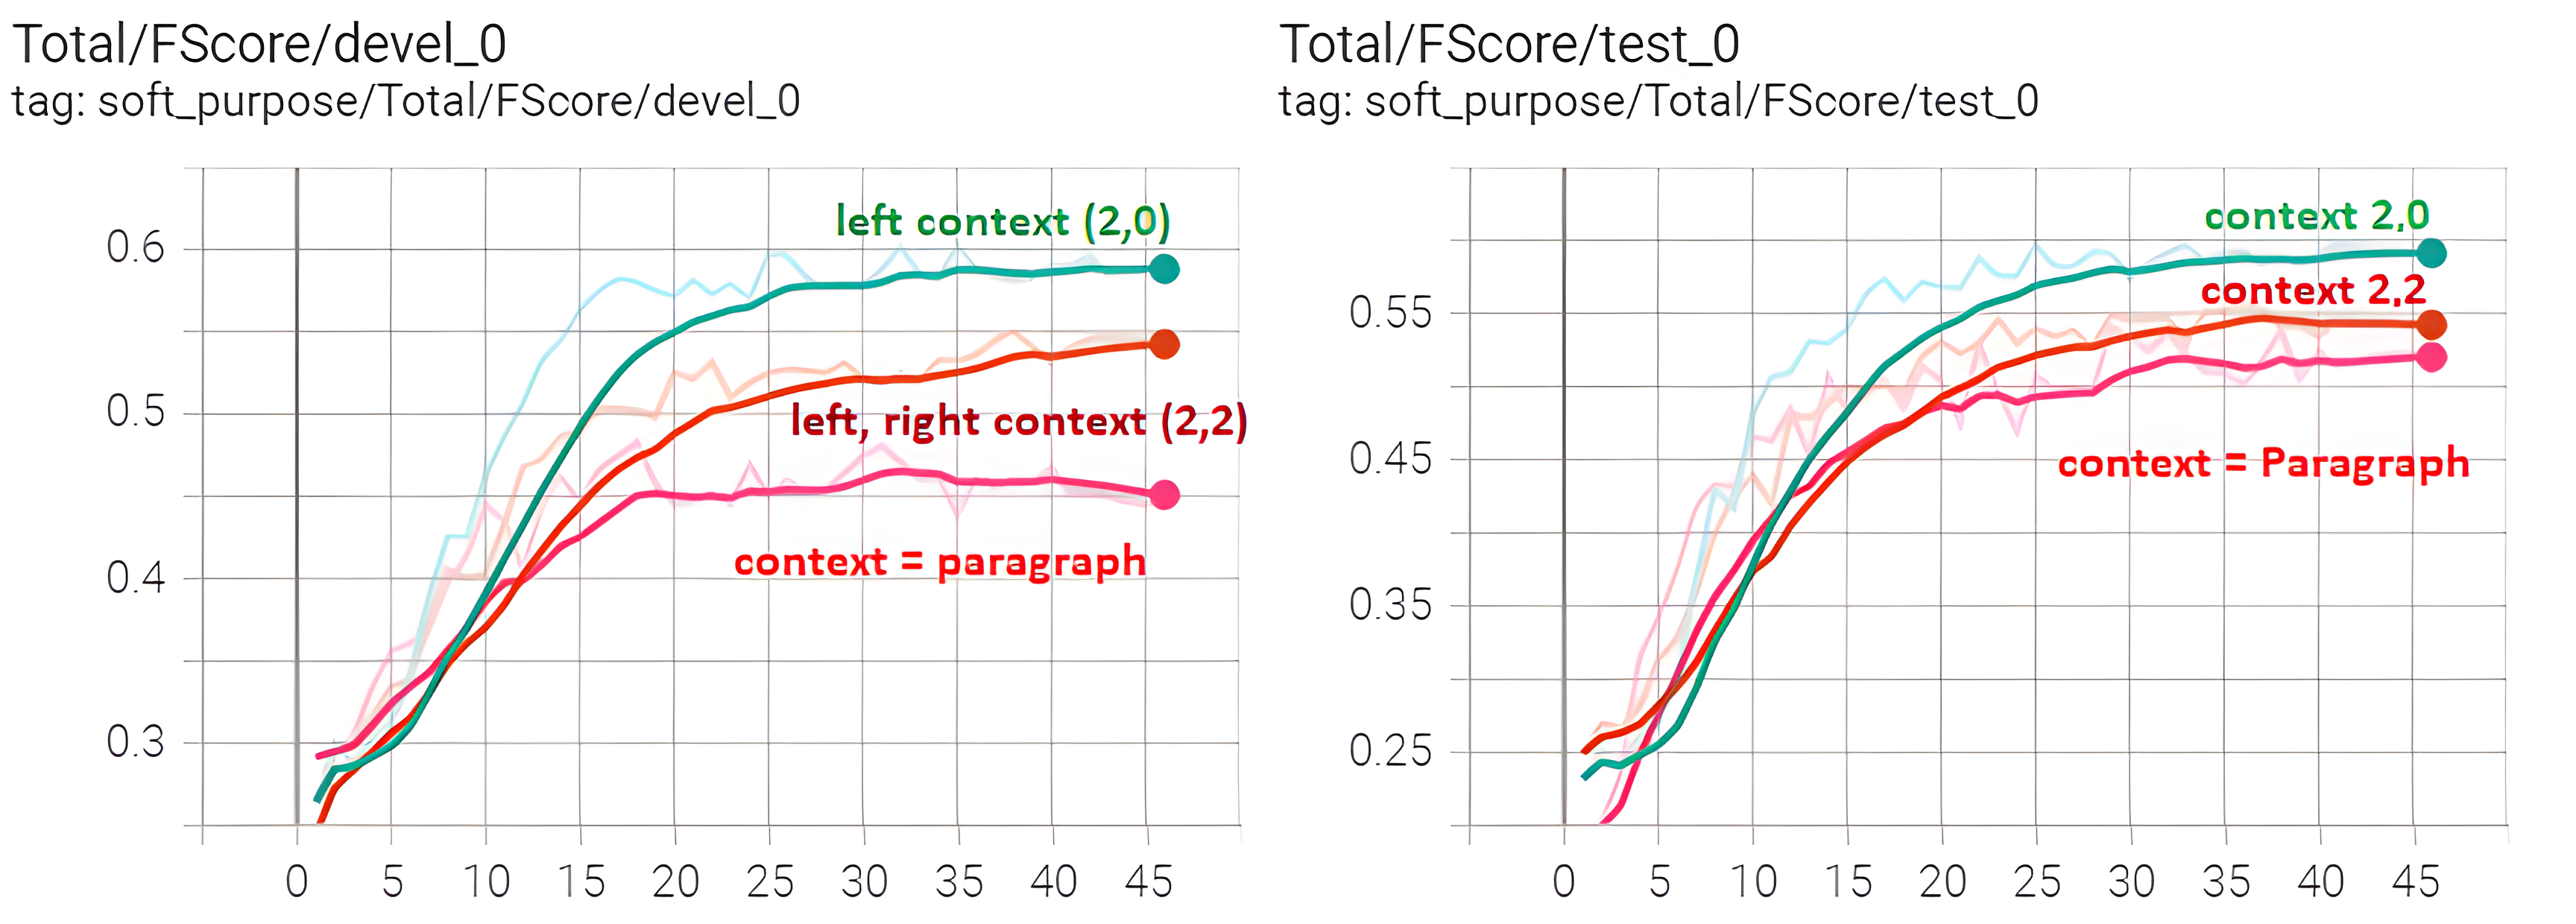
\includegraphics[width=.90\textwidth]{4.graphics/figures/ch_6/2.left_context_vs_right/HD/context_paragrapgh}
	\caption{Software purpose classification (Total) F1-score performance for devl. set (left) and test set (right) deteriorates when very large context, paragraph, is considered.}
	\label{fig:chapter06:whole_par}
\end{figure}


\subsection{Context Outside a Paragraph}
\label{sec:chapter06:contxtOutside}


The other scenario considered was evaluation of software purpose classification performance when context is not limited within a paragraph. Accordingly, classification performance with 2 adjacent sentences with in a paragraph is compared with context information of 2-adjacent sentences regardless of their position in the paragraph. \\

According to the classifier's F-score, software purpose classification degraded when a context is not limited within a paragraph as shown on the figure 6.6. This agrees with the fact that each paragraph of a scientific publication conveys a specific information and a contextual information outside a paragraph is not useful for the classifier.  The Sci-BERT classifier model which considers context outside a paragraph is listed at the git-hub\footnote{\url{https://github.com/BeTKH/SoMeNLP/tree/contxt_out_parg}}. \\

\begin{figure}[htbp]
	\centering
	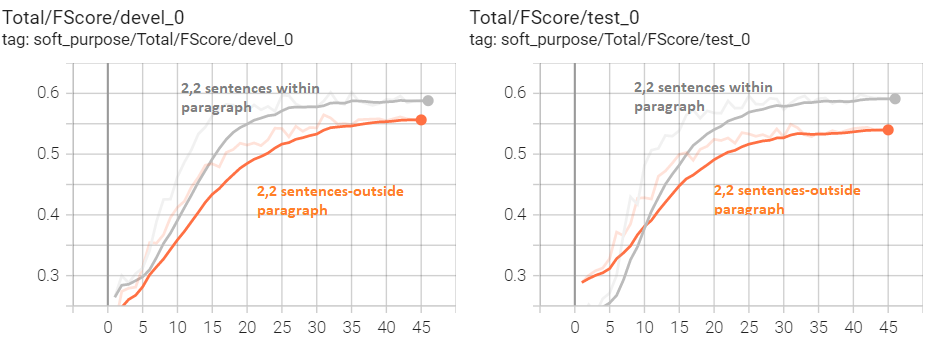
\includegraphics[width=.80\textwidth]{4.graphics/figures/ch_6/2.left_context_vs_right/HD/Fscore_outside_paragrapgh_vs_inside}
	\caption{Software purpose classification (Total) F1-score performance for devel. set (left) and test set (right) did not benefit from context outside a paragraph. }
	\label{fig:chapter06:with}
\end{figure}


Based on evaluation of software purpose classifier's performance, overall it was observed that left context is more important than the right context. In addition, it was observed that context from both left and right as well as a broader context outside a paragraph did not improve the classification performance. \\

Based on results, shown on figure 6.6, for all subsequent steps of software-purpose classification model evaluation, only two adjacent sentences from the left context are considered. \\


\section{Classification with 2-Cascade Sci-BERT}
\label{sec:chapter06:2lc}

The 4-cascade \ac{Sci-BERT} multi-class classifier model, shown on the figure 5.6, has been used for the software purpose classification until this point. This model, not only classifies software usage purposes but also other information about software such as software as an application, software types, and mention-types. \\


Overall the 4-cascade \ac{Sci-BERT} classifier’s performance has been poor regardless of consideration of various factors discussed above. For this reason, it was desired to study weather the removal of intermediate classifier modules would improve software purpose classification. Consequently, \emph{software-type} and \emph{mention-type} classifier modules, have been removed resulting into a 2-cascade classifier-module as shown on the figure 6.7. The \emph{software-entity} classifier module, however, is kept because identification of software would assist software purpose classification.  \\

\begin{figure}[htbp]
	\centering
	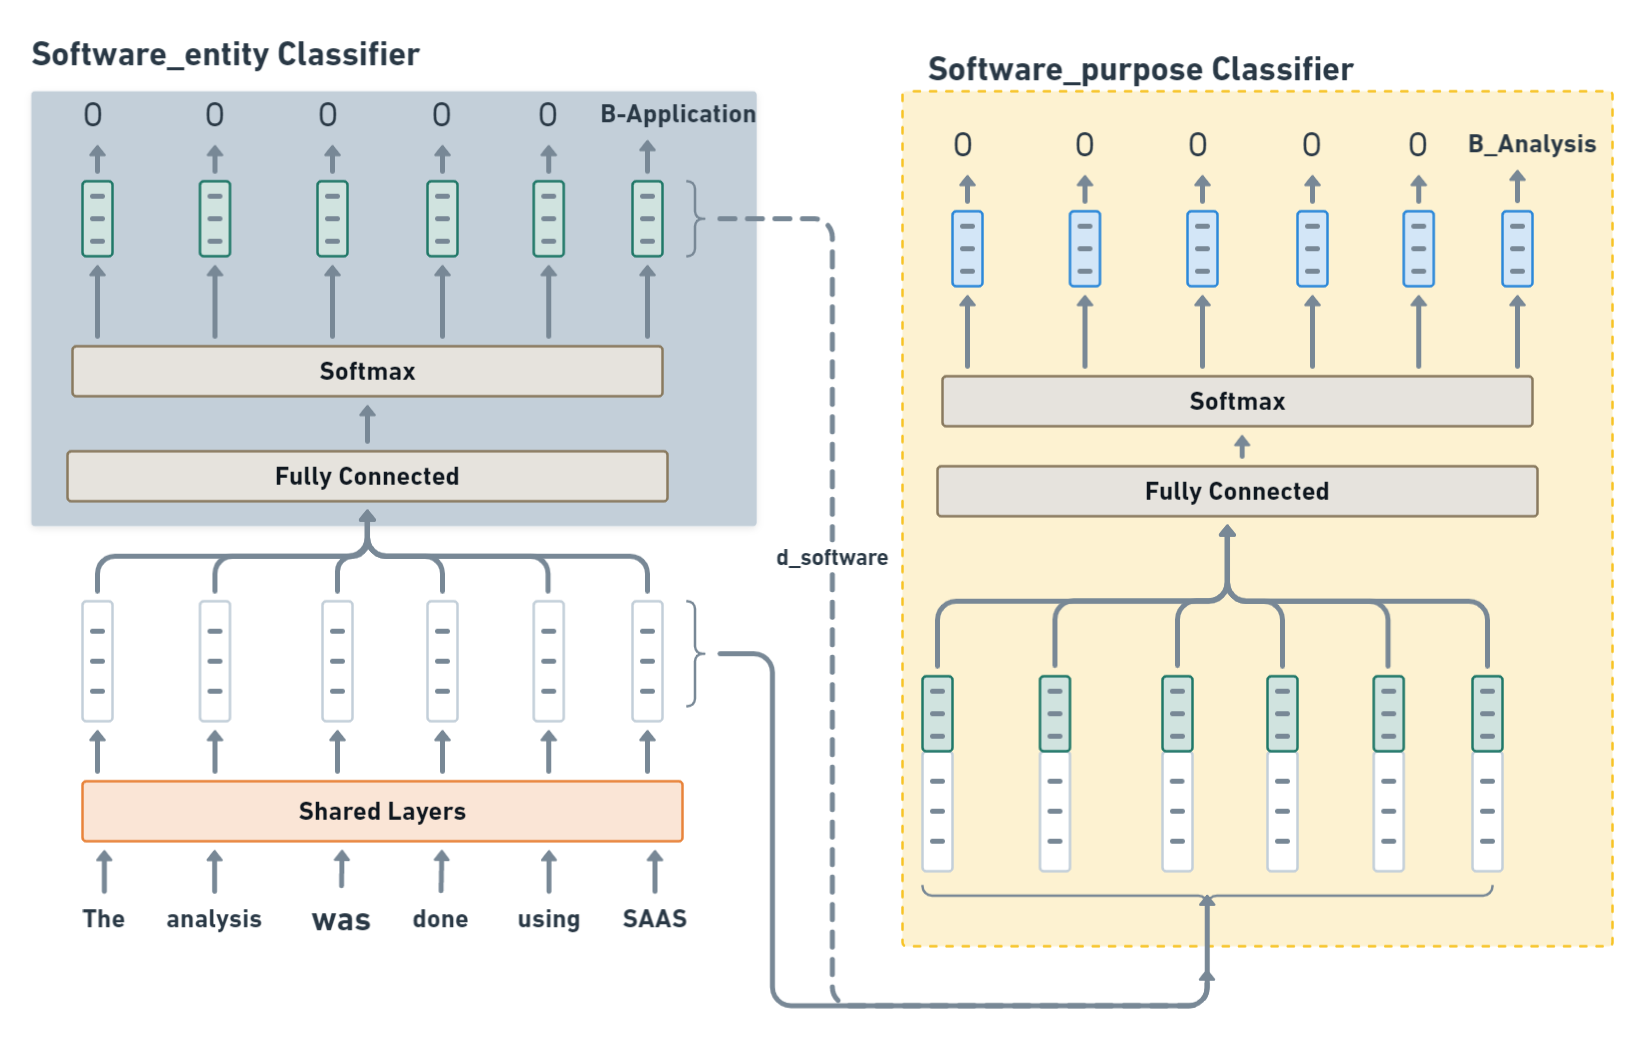
\includegraphics[width=.65\textwidth]{4.graphics/figures/ch_5/2LC}
	\caption{Fully connected, 2-cascade \emph{software-entity} and \emph{software-purpose} classifier model.}
	\label{fig:chapter06:2lc}
\end{figure}

Evaluation of the 2-cascade Sci-BERT classifier model reveals that overall \emph{software purpose} classification F-score has shown small improvement compared to the original 4-cascade classifier  \ac{Sci-BERT} model, where as the \emph{software-entity} classifier’s performance does not indicate any performance improvement as shown in figures 6.8 and 6.9 respectively. Comparison of software purpose classification performance in terms of F-score (F), Precision (P) and Recall (R) for 2-Cascade Sci-BERT classifier versus 4-cascade Sci-BERT classifier is shown on the table 6.3. \\

\begin{figure}[htbp]
	\centering
	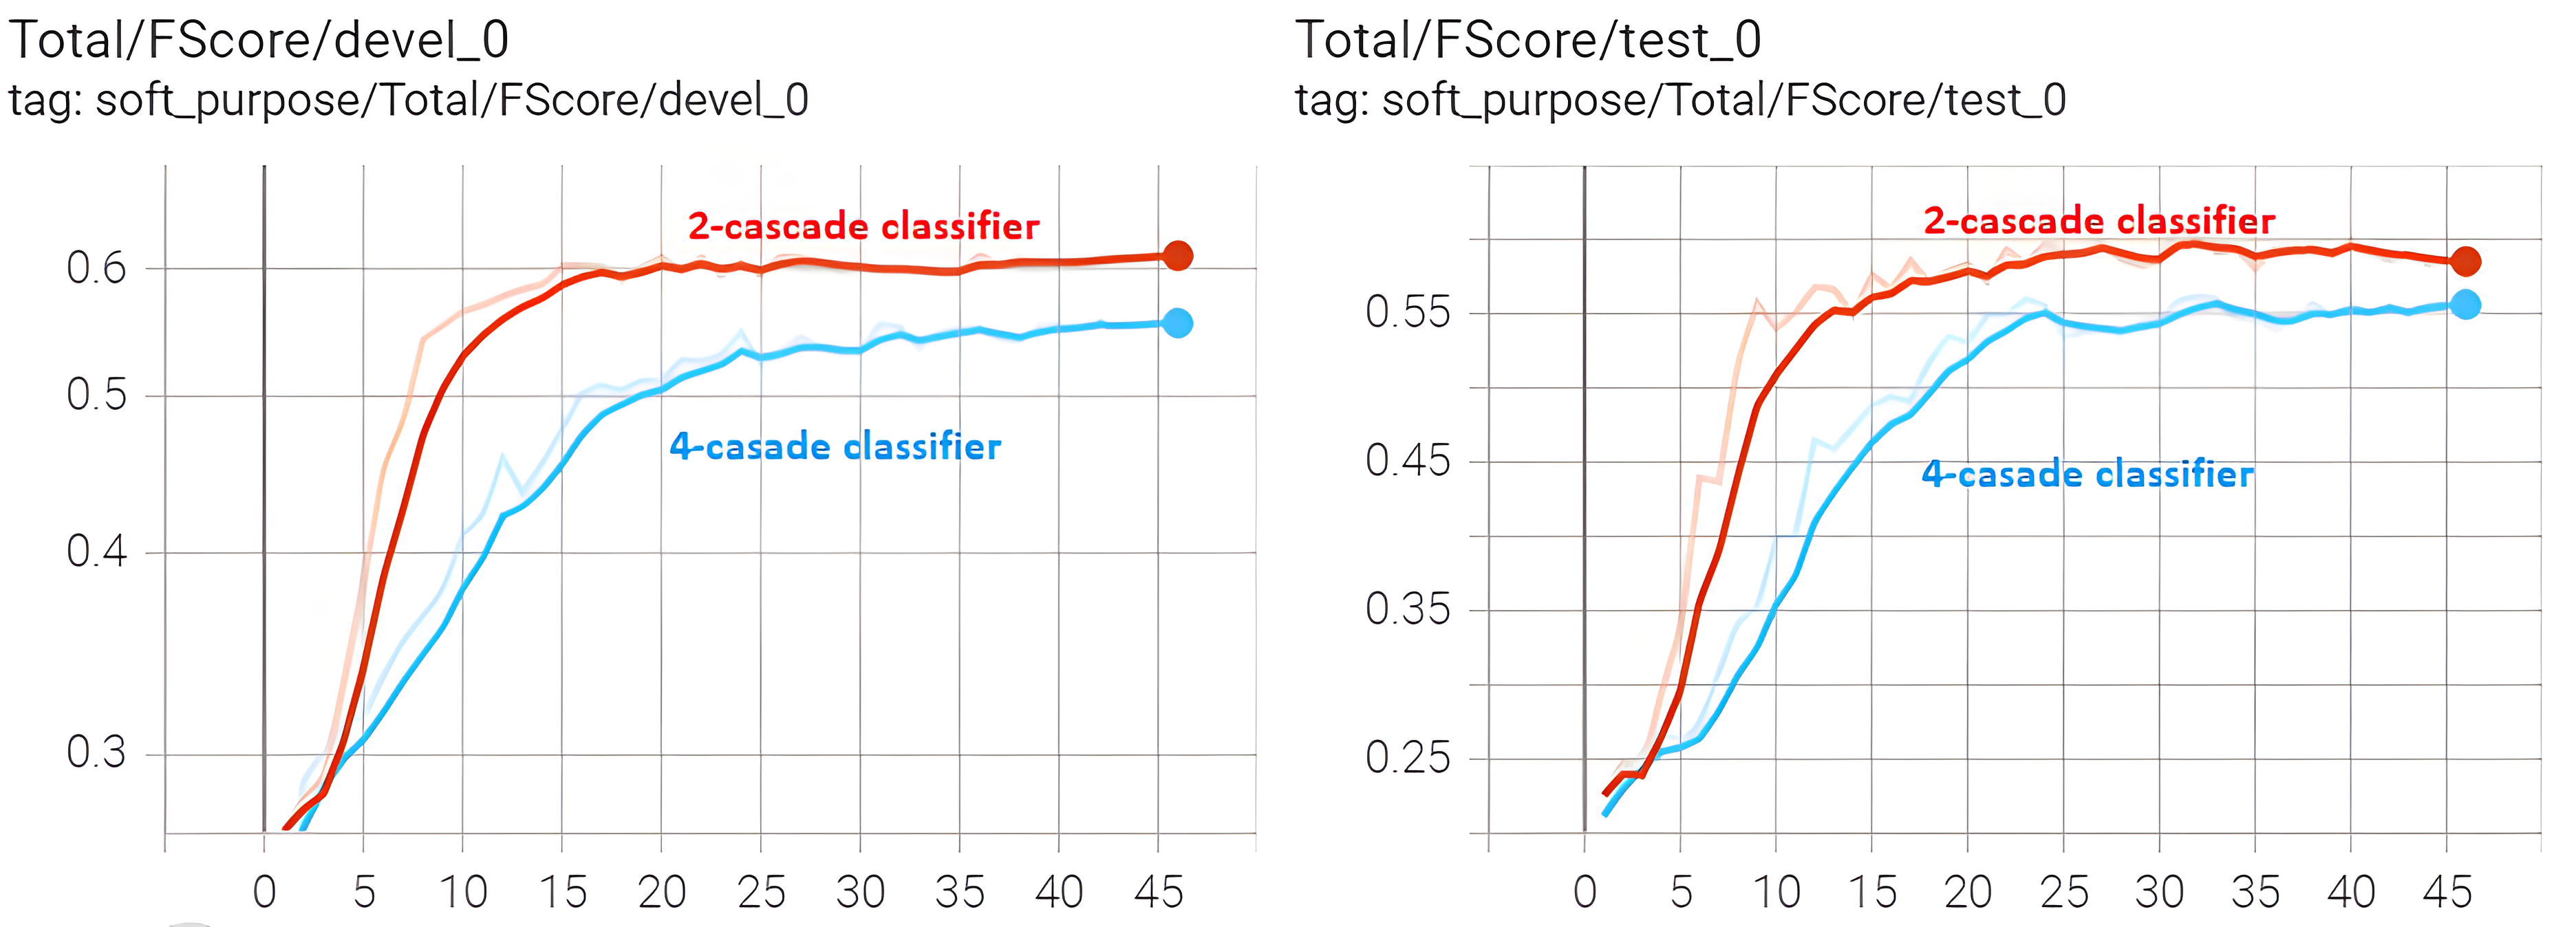
\includegraphics[width=1\textwidth]{4.graphics/figures/ch_6/5.2layerClassifier/HD/4casadeVs2cascade}
	\caption{2-cascade classifier has slightly better (Total) F-score over devl. set(left) and test set(right) for software \emph{purpose classification}.}
	\label{fig:chapter06:with}
\end{figure}

\begin{table}[ht]
	\centering
	\caption{Evaluation of software purpose classifier's performance with 2-cascade Sci-BERT model (2C) versus 4-cascade Sci-BERT model (4C) shows that the 2C-model has slightly better performance compared to 4C-model.}
	\begin{tabular*}{.90\textwidth}{@{\extracolsep{\fill}}  l  l l  l r r } %l left align , c- center
		\hline
		Software Purpose & Metric & Dev.(2C)        & Dev.(4C)     & Test.(2C)  &Test(4C) \\
		\hline 
		Analysis        & F     & 0.72        & 0.69     &0.69     &0.68   \\
		& P     & 0.73        & 0.68     &0.65     &0.64   \\
		& R     & 0.71        & 0.70     &0.74     &0.73   \\
		\hline
		Data-Collection  & F     & 0.34        &  0.24    & 0.35    & 0.25  \\
		& P     & 0.36        &  0.23    & 0.41    & 0.20  \\
		& R     & 0.32        &  0.25    & 0.31    & 0.25  \\		
		
		\hline
		Pre-Processing   & F     & 0.49        &  0.39    & 0.57    & 0.55  \\
		& P     & 0.40        &  0.32    & 0.48    & 0.46  \\
		& R     & 0.61        &  0.50    & 0.68    & 0.73  \\
		\hline
		Modeling         & F     & 0.64        &  0.47    & 0.43    & 0.38  \\
		& P     & 0.57        &  0.48    & 0.42    & 0.38  \\
		& R     & 0.71        &  0.46    & 0.44    & 0.38  \\
		
		\hline
		Programming      & F     & 0.41        &  0.46    & 0.32    & 0.37  \\
		& P     & 0.32        &  0.36    & 0.28    & 0.32  \\
		& R     & 0.55        &  0.55    & 0.38    & 0.44  \\
		
		\hline
		Simulation      & F     & 0.28        &  0.28    & 0.00    & 0.00 \\
		& P     & 0.66        &  0.64    & 0.00    & 0.00  \\
		& R     & 0.18        &  0.18    & 0.00    & 0.00  \\
		
		\hline
		Stimulation     & F     & 0.50        &  0.48    & 0.25    & 0.23 \\
		& P     & 0.56        &  0.52    & 0.21    & 0.29  \\
		& R     & 0.44        &  0.45    & 0.31    & 0.20  \\
		
		\hline
		Visualization   & F     & 0.60        &  0.45    & 0.69    & 0.57  \\
		& P     & 0.59        &  0.43    & 0.62    & 0.56  \\
		& R     & 0.61        &  0.47    & 0.78    & 0.59  \\
		\hline
		Total 	& F     & 0.61*        &  0.55    & 0.56*    & 0.55  \\
		& P     & 0.61*        &  0.51    & 0.54*    & 0.52  \\
		& R     & 0.62*        &  0.58    & 0.64*    & 0.60  \\
		\hline
	\end{tabular*}
\end{table}%


\begin{figure}[htbp]
	\centering
	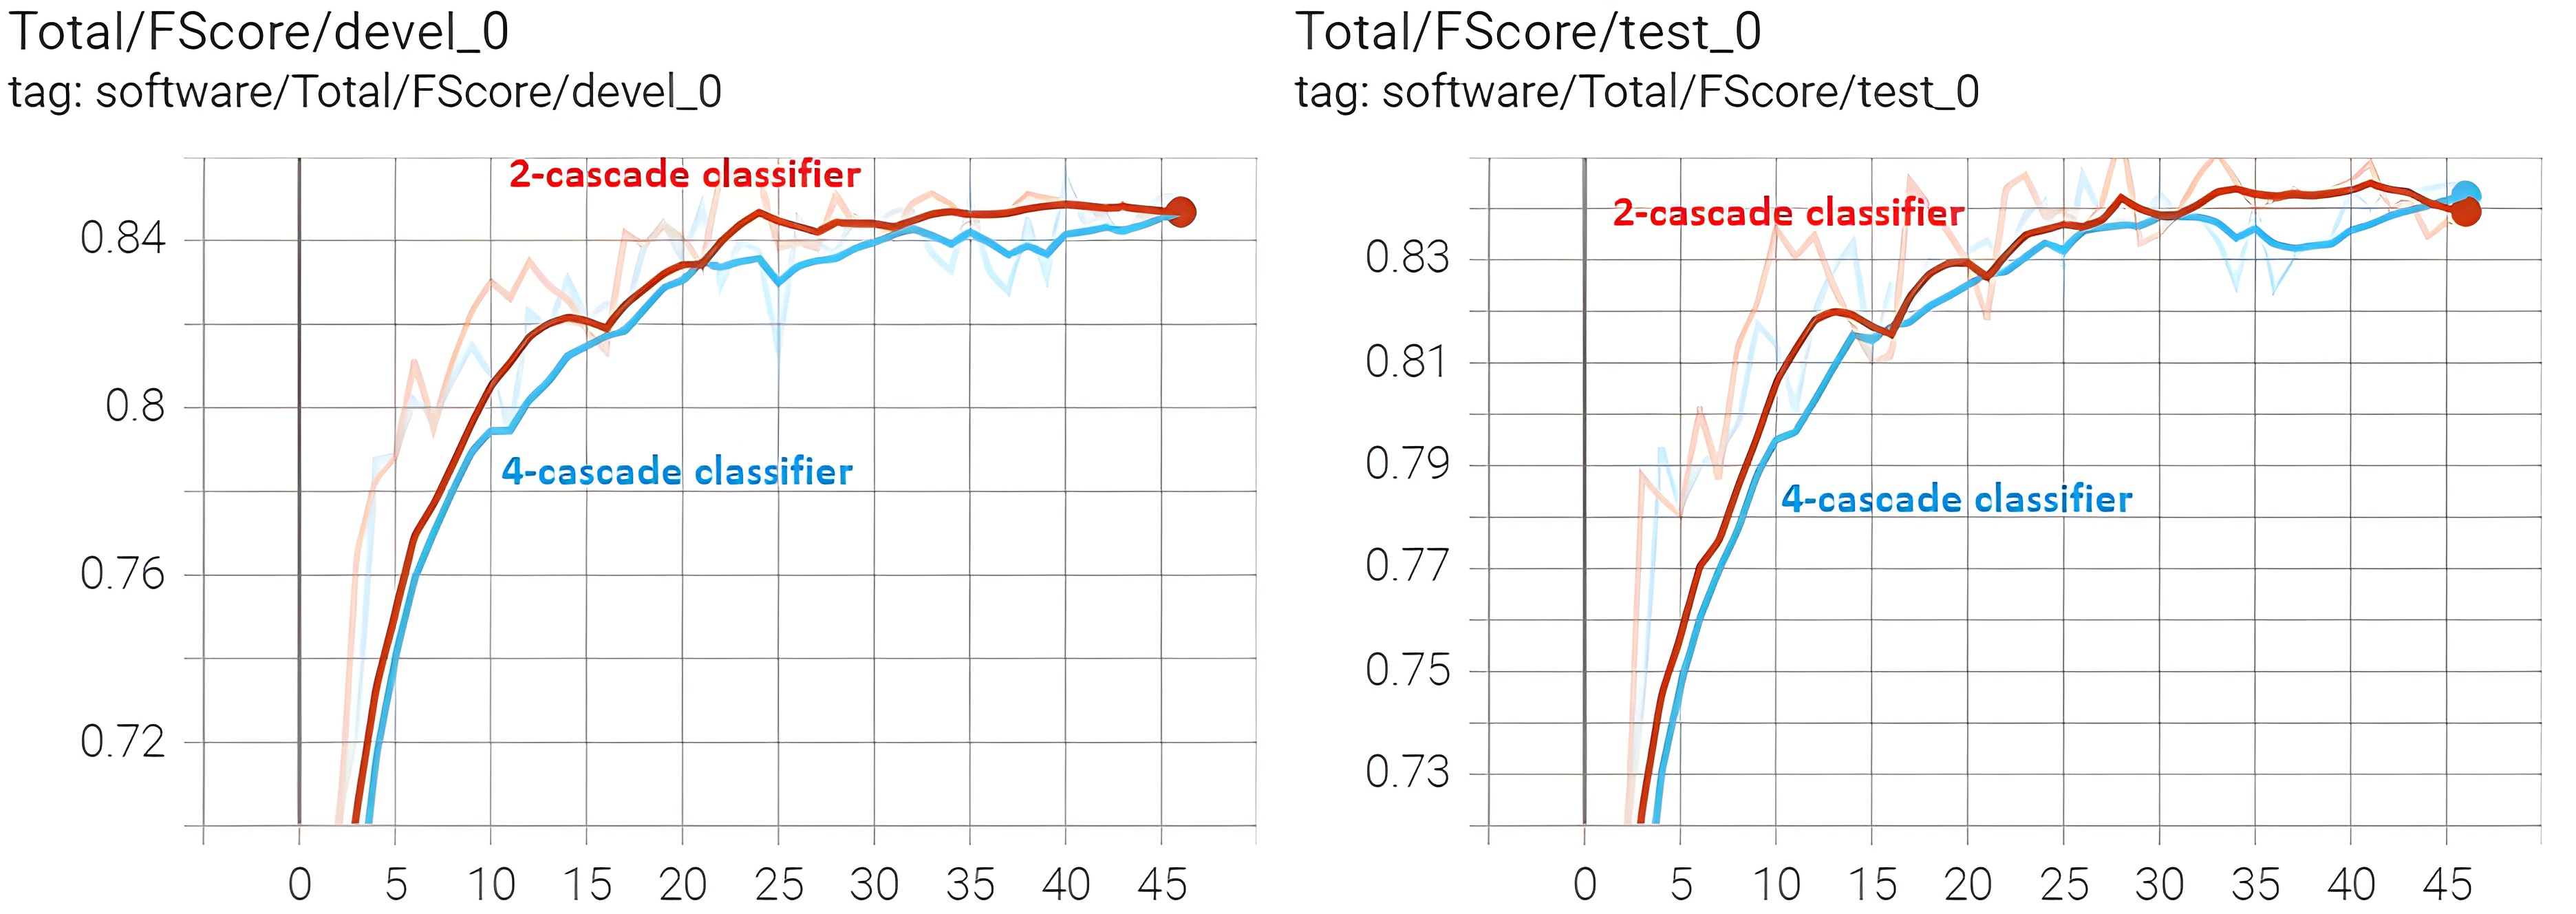
\includegraphics[width=1\textwidth]{4.graphics/figures/ch_6/5.2layerClassifier/HD/4casadeVs2cascade_software}
	\caption{2-cascade classifier has no significant performance improvement in terms of (Total) F-score over devl. set(left) and test set(right) for \emph{software classification}.}
	\label{fig:chapter06:with}
\end{figure}

The evaluation of classifier’s performance by removing the intermediate classifier modules from the 4-cascade model gives a marginal improvement for \emph{software purpose} classification, but not for \emph{software-entity} classification. This might point out, probably flawed classifications of intermediate layers might have an impact on the software purpose classifier which lies at the end of the classification cascade. \\

Since a 2-cascade Sci-BERT \emph{software-purpose} classifier has slightly better performance, for the next steps this model has been used. \\

\section{Bio-BERT vs Sci-BERT}
\label{sec:chapter06:biosci}

As mentioned before, on section 5.3.1, the other variant of BERT model which is trained with SoMeSci dataset, in this thesis , is Sci-BERT. Even though both \ac{Bio-BERT} and \ac{Sci-BERT} give a contextualized representation of a word in a sentence, representations of a word would differ due to the inherent difference of corpora used for pre-trained models of Bio-BERT and Sci-BERT \citep{beltagy2019scibert,li2019fine}. For this reason, a 2-cascade classifier model has been trained with Bio-BERT and results are compared with Sci-BERT model. \\

Among various varieties of Bio-BERT models, Bio-BERT(base) and Bio-BERT(large) models have been trained with SoMeSci dataset to compare performance with Sci-BERT model. \\

The results of evaluation indicate that  Bio-BERT-large\footnote{\url{https://huggingface.co/dmis-lab/biobert-large-cased-v1.1}} model performed slightly better than the Sci-BERT\footnote{\url{https://huggingface.co/allenai/scibert_scivocab_cased}} model according to the total F-score. However, Sci-BERT has superior performance compared to the Bio-BERT-base\footnote{\url{https://huggingface.co/dmis-lab/biobert-base-cased-v1.2}} model. \\

\begin{figure}[htbp]
	\centering
	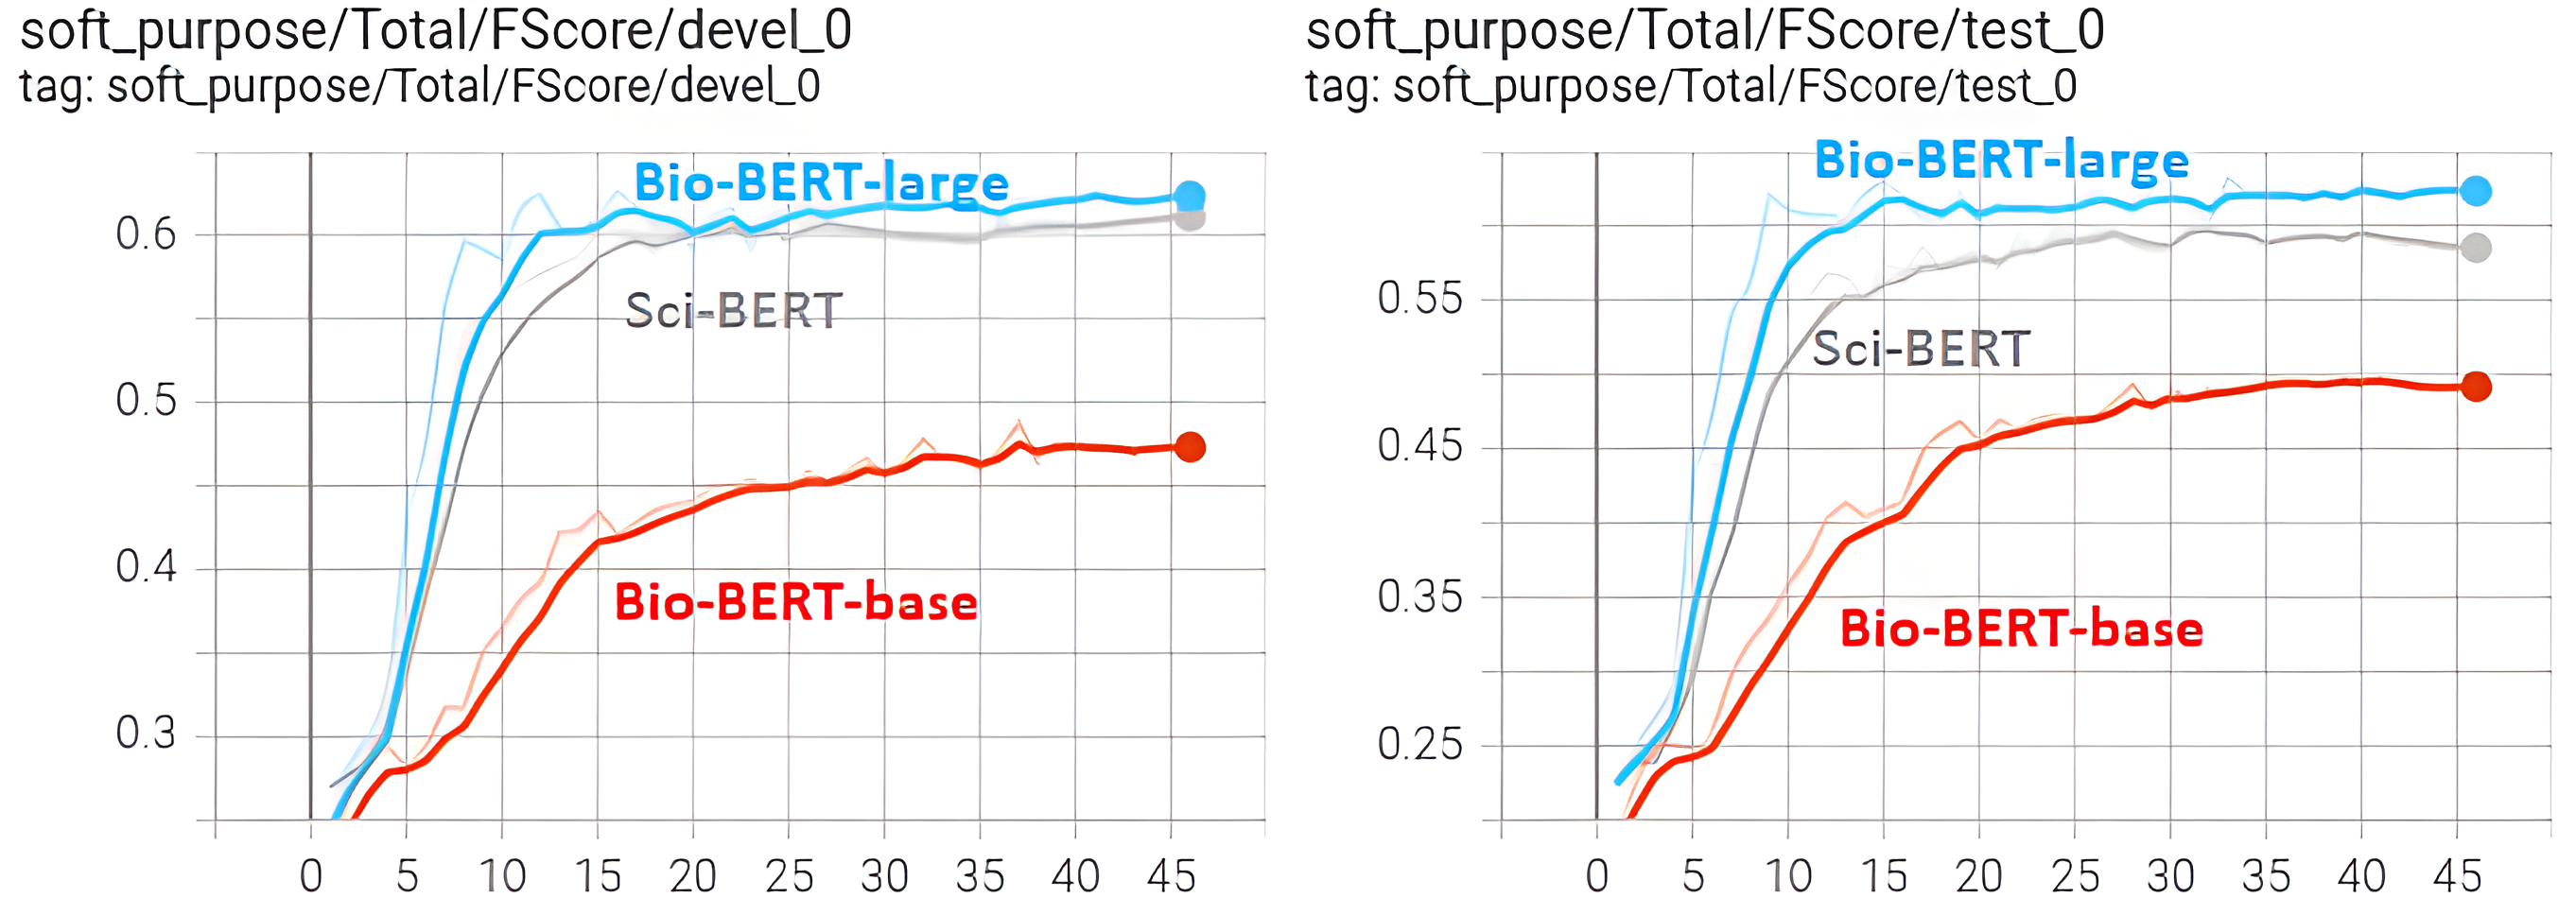
\includegraphics[width=1\textwidth]{4.graphics/figures/ch_6/6.BIoBERT_vs_SCIBERT_2LAYER_Classifier/HD/BIobert-large-small-cybert}
	\caption{2-Cascade \emph{software-purpose} classifier, trained with Bio-BERT-large, Sci-BERT and Bio-BERT-base indicates that the Bio-BERT-large has superior (Total) F-score over Sci-BERT as well as Bio-BERT-base when tested with devl-set(left) and test-set(right).}
	\label{fig:chapter06:with}
\end{figure}


Even though Bio-BERT-large software purpose classifier has slightly better total F-score, the model was too slow during a training. The Sci-BERT 2-cascade \emph{software-entity} and \emph{software-purpose} classifier model gives reasonable classification performance with a relatively fast training.  






















